\documentclass[12pt]{article}
\usepackage[left=1in, right=1in, top=1in, bottom=1in]{geometry}
\usepackage{graphicx}
\usepackage{url}
\usepackage{cite}
\usepackage{float}
\usepackage{caption}
\usepackage{subcaption}
\usepackage{hyperref}
\hypersetup{
    colorlinks,
    citecolor=black,
    filecolor=black,
    linkcolor=black,
    urlcolor=black
}

\renewcommand{\familydefault}{\sfdefault}


\begin{document}
\begin{titlepage}
    \begin{center}
        \LARGE
        \textbf{ELE 402 - GRADUATION PROJECT II}

        \Large
        \textbf{INTERIM REPORT}

        \vspace{70pt}

        \textit{
            Hacettepe University \\
            Department of Electrical and Electronics Engineering
        }
    \end{center}

    \vspace{90pt}

    \large

    \textbf{Project Title:} Sensor Fusion in the Cloud \\

    \textbf{Project Group Members:} Ertuğrul Tiyek, Ahmet Yusuf Şirin

    \vspace{30pt}

    \textbf{Project Supervisor:} Asst. Prof. Dr. İsmail Uyanık \\

    \textbf{Submission Date:} 07.05.2023

    \vspace{\fill}

    \begin{center}
        \textit{SPRING 2022-2023}
    \end{center}
\end{titlepage}

\clearpage

\tableofcontents
\listoffigures
\listoftables

\clearpage

\begin{abstract}
    One of the most important aim of the modern technology is the sensing the environment. Living beings have sense organs to know the environment. They have brains to make fusion the sensor data and augment the environmental information taken from sense organs. For example, human standing in balance, we can say that they use the data coming from their eyes and ears together.

    People are studying to make this sensing and augmenting artificially, too. They use computers to achieve this. But computers cannot sense the environment directly. They need some devices called sensors. There are all kinds of sensors to measure different environmental quantities. For same quantity, there are different sensors using different technologies, have different precision and accuracy levels. Each sensor has its advantages and disadvantages. Even sensors that are serving a different purpose can help to augment same information other than their main. This is known as "sensor fusion"~\cite{enwiki:1115352853}. Just like humans, robots are use camera and inertial sensors to stand in balance. 

    In our project, sensor fusion handles extracting depth information. Sensor fusion can be implemented using specific algorithms like EKF, CNN etc. according to quantity that will be calculated, number and types of sensors used, accuracy and performance needed. We are planning to develop a sensor fusion algorithm with the help of living organisms. As we mentioned before, living beings perform sensor fusion perfectly. We will be examining the zebra fish and how it processes data of its sense organs to produce depth information. Then we will try to develop similar algorithm or improve our algorithm with data taken from zebra fish. 

    Depth information can be used for many applications like automatic driven vehicles, UAVs, Augmented Reality devices and 3D modeling of areas. Our concept in this project will be autonomous controlled SLAM Robot. Simultaneous localization and mapping (SLAM) is the computational problem of constructing or updating a map of an unknown environment while simultaneously keeping track of an agent's location within it~\cite{enwiki:1120084976}. We use a robot to move the system. 

    Another concept we aim to use is cloud computing. Mobile computing devices may not match the performance requirements in some cases. To achieve more accurate depth information, complex control algorithms or neural networks will be used in our project which needs high computing power. As an alternative to the mobile computing devices, we may use cloud computing.  

    From the point on we are studying on the sensor fusion. In this report we will briefly emphasize the legged robot usage for our final decisions. On the other hand, the concept ot the sensor fusion and the alternative methodologies to implement it correctly to serve the main purpose of sensor fusion, that is reliable odometry data extraction.
\end{abstract}

\section{INTRODUCTION}

This report presents the progress and design iterations of a fully ROS-based robot, focusing on sensor fusion and SLAM operations. The project aims to develop a robotic platform capable of autonomously navigating and mapping an environment with the help of a variety of sensors. The purpose of this report is to provide an overview of the prototype design and the design process, highlighting the key features, testing results, and evaluations from each iteration. This document is intended to serve as a guide for future work and improvements on the project.

The report is organized as follows: Section 2 introduces the prototype, including its purpose, functionalities, and key features. Section 3 details the design process, covering the different iterations carried out to refine the prototype, along with their respective testing and evaluation.

\section{PROTOTYPE}

The prototype developed for this project is a fully ROS-based robot designed to perform sensor fusion and SLAM operations. The primary purpose of building this prototype is to demonstrate the effectiveness of integrating various sensors for accurate and efficient mapping and navigation in an unknown environment. The prototype serves as a platform for testing different sensor fusion algorithms and SLAM techniques to identify the most suitable combination for real-world applications.

The prototype consists of a mobile robotic base equipped with multiple sensors, including LiDAR, camera, inertial measurement unit (IMU), and wheel encoders. These sensors work in tandem to gather data from the environment, which is then processed and combined using sensor fusion algorithms. The fused data is fed into the SLAM system, allowing the robot to construct a map of its surroundings while simultaneously keeping track of its position within that map.

Key features of the prototype include:

\begin{enumerate}
    \item ROS integration: The robot's software architecture is built on the Robot Operating System (ROS), a widely used, flexible framework for robotics development. This allows for easy integration of existing ROS packages and ensures compatibility with a wide range of sensors and algorithms.

    \item Sensor fusion: The prototype employs various sensor fusion techniques to combine the data from different sensors, resulting in a more accurate and robust representation of the environment. This helps improve the robot's overall performance in mapping and navigation tasks.
    
    \item SLAM implementation: The prototype integrates state-of-the-art SLAM algorithms to simultaneously localize the robot within the environment and construct a map based on the fused sensor data. This enables the robot to navigate autonomously and efficiently, even in previously unexplored areas.
    
    \item Modular design: The hardware and software components of the prototype are designed to be modular, allowing for easy modification, replacement, and upgrading of individual elements. This ensures that the robot can be easily adapted to accommodate new sensors or algorithms as they become available.
\end{enumerate}

LOAM (Lidar Odometry and Mapping) is a state-of-the-art algorithm for simultaneous localization and mapping (SLAM) that leverages the advantages of lidar sensors. The LOAM algorithm is designed to work in real-time and has been widely adopted in various robotic applications, including autonomous vehicles and drones, due to its robust performance and high accuracy.

The main idea behind LOAM is to separate the point cloud data generated by the lidar sensor into two components: ground points and edge points. Ground points represent the flat surfaces of the environment, while edge points correspond to the sharp features such as corners and edges. By analyzing the relative motion of these two sets of points, LOAM can estimate the robot's pose and build a detailed map of the environment.

LOAM is particularly well-suited for robotic platforms equipped with high-resolution lidar sensors, as it can handle large amounts of data efficiently and maintain accurate localization even in complex environments. Integrating LOAM into the prototype enables the robot to perform SLAM tasks with high precision, making it an ideal choice for the sensor fusion system.

\begin{figure}[h]
    \centering
    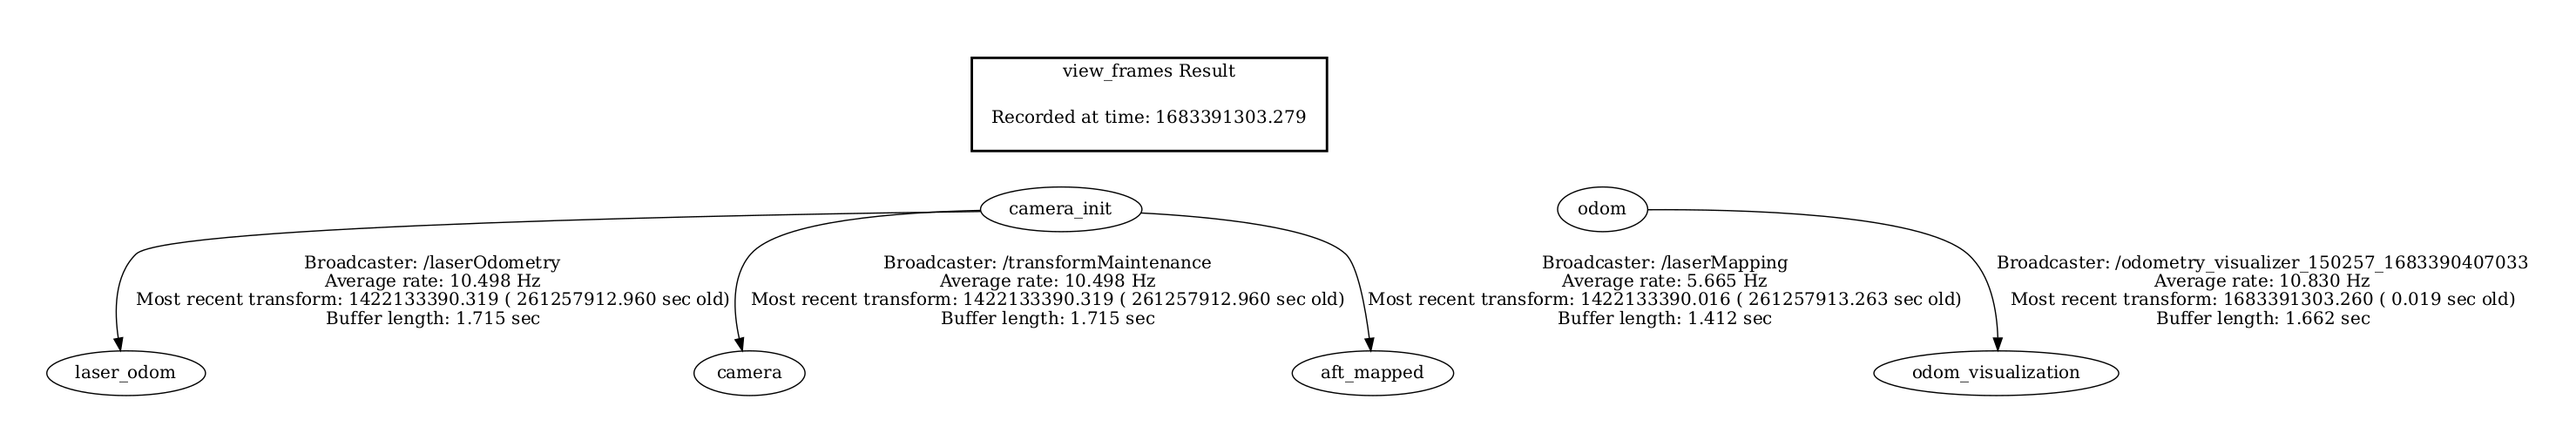
\includegraphics[width=0.9\textwidth]{loam_ros_graph.png}
    \caption{Local Host LOAM ROS Node/Topic Schematic}
\end{figure}

The Robot Operating System (ROS) is a flexible and powerful framework for developing robotic applications, providing a wide range of libraries, tools, and software components for various robotic tasks. Running ROS on a Raspberry Pi (RPI) is an efficient and cost-effective way to create a compact, versatile robotic system that can take advantage of ROS's capabilities.

By utilizing an RPI as the central processing unit for the robot, the system can benefit from the RPI's low power consumption, small form factor, and extensive community support. This allows for a lightweight, portable robotic platform that can be easily extended and customized according to specific application requirements. Moreover, the RPI can run a Linux-based operating system, which is compatible with ROS, making it an ideal choice for integrating ROS into the robot's control system.

Installing and running ROS on an RPI involves setting up the necessary dependencies, configuring the ROS environment, and deploying the desired ROS packages. Once the ROS system is up and running on the RPI, the robot can utilize various ROS functionalities, such as communication between different nodes, sensor data processing, and control algorithms implementation.

Integrating ROS with the RPI enables seamless communication with other hardware components, such as sensors and actuators, through the use of ROS topics, services, and actions. This allows for efficient sensor fusion, SLAM operations, and overall system coordination. The combination of ROS and RPI offers a powerful, compact solution for developing advanced robotic applications while maintaining a low-cost and accessible platform.

\begin{figure}[h]
    \centering
    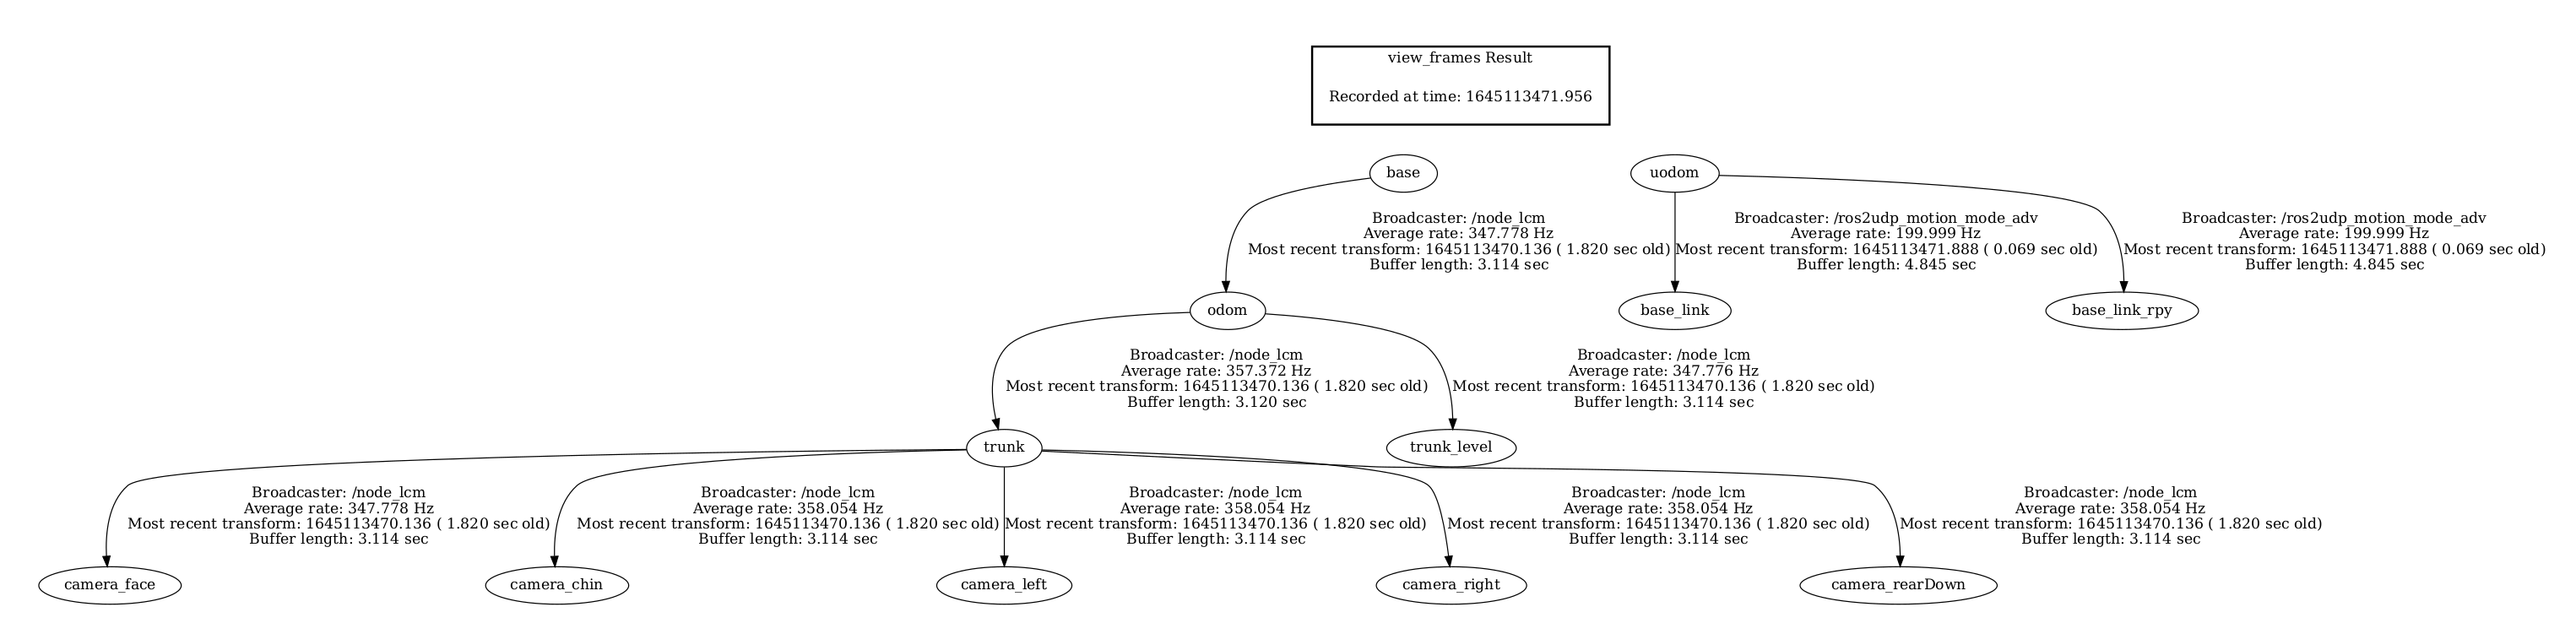
\includegraphics[width=0.9\textwidth]{rpi_ros_graph.png}
    \caption{Legged Robot RPi ROS Node/Topic Schematic}
\end{figure}
    
\section{DESIGN PROCESS}

The design process of the prototype followed an iterative approach, involving multiple stages of development, testing, and evaluation. This methodology allowed the team to identify shortcomings in the initial design, implement modifications, and continuously improve the prototype's performance. Each iteration focused on addressing specific challenges, refining the sensor fusion techniques, and optimizing the SLAM implementation. In the following subsections, we present the steps of the design process performed in constructing the prototype, including the objectives, testing, results, and evaluation for each iteration.

    \subsection{ITERATION 1: INITIAL SENSOR INTEGRATION AND ROS SETUP}
    
    The first iteration aimed to establish a solid foundation for the project by integrating the different sensors and setting up the ROS framework for the robot. The main objectives of this iteration were:

    \begin{enumerate}
        \item Selection and integration of appropriate sensors (LiDAR, camera, IMU, and wheel encoders) for the robot.
        \item Installation and configuration of ROS on the robot's embedded computer system.
        \item Setup of the communication infrastructure between the sensors, ROS nodes, and the robot's control system.
    \end{enumerate}

    In addition to the aforementioned advantages, the integration of the Raspberry Pi (RPI) with the Robot Operating System (ROS) allows for enhanced communication capabilities with micro-ROS systems. Micro-ROS is a lightweight version of ROS specifically designed for microcontrollers, enabling resource-constrained devices to become part of the ROS ecosystem. By incorporating micro-ROS into the system, it becomes possible to extend the functionality and modularity of the robotic platform even further.

    The RPI serves as the central communication hub between the ROS nodes and the micro-ROS system. It manages the flow of data between the different subsystems and ensures seamless interaction among the various components of the robot. To facilitate this communication, the RPI is connected to a network switch, which enables efficient data transmission and distribution throughout the system.

    The network switch plays a crucial role in the overall performance and reliability of the robotic system. It ensures that all components, including the RPI, micro-ROS nodes, and other connected devices, can exchange information effectively and maintain synchronized operation. By leveraging a network switch in conjunction with the RPI, the system can handle multiple data streams, balance network traffic, and reduce latency, thereby improving the overall performance of the robot.

    In summary, the combination of the Raspberry Pi, ROS, micro-ROS, and a network switch provides a powerful and versatile robotic platform. The RPI acts as the central processing unit and communication hub, allowing for efficient coordination between the ROS nodes and micro-ROS systems. The use of a network switch ensures seamless data exchange among the various components of the robot, resulting in a robust, scalable, and high-performance robotic system capable of tackling a wide range of applications.

    \begin{figure}[H]
        \centering
        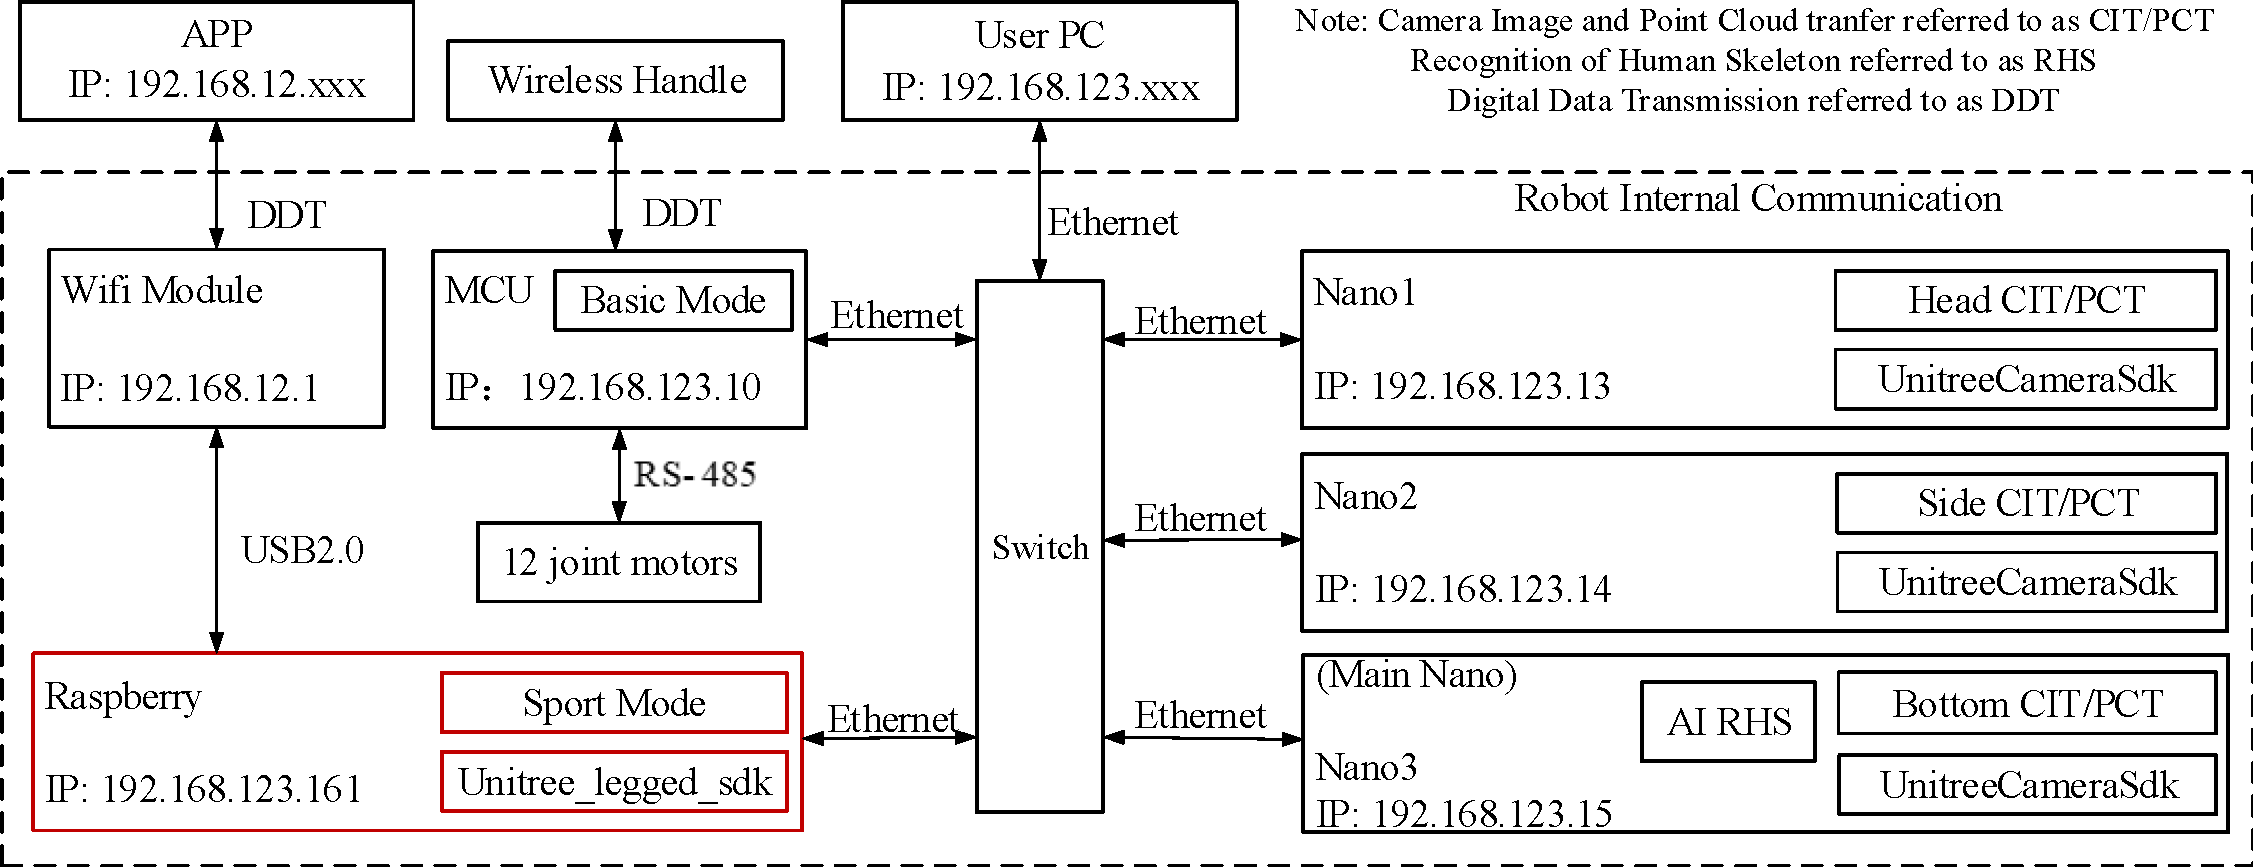
\includegraphics[width=0.9\textwidth]{Go1CommFram_E.png}    
        \caption{Infrastructure of the Unitree Go1 Robot}
    \end{figure}

        \subsubsection{TESTING AND RESULTS}

        The robot's hardware and software components were assembled, and the integration of sensors with the ROS framework was tested. The communication between the sensors and ROS nodes was verified using the provided visualization tools (such as RViz) to ensure proper data flow. Preliminary tests were conducted to evaluate the robot's ability to gather data from the environment using the sensors.

        \subsubsection{EVALUATION}

        The results from the first iteration revealed the successful integration of sensors and the establishment of the ROS environment. However, some issues were identified, such as occasional data loss due to communication bottlenecks and the need for better synchronization between the sensors. These issues were noted and addressed in the subsequent iterations.

    \subsection{ITERATION 2: SENSOR FUSION AND SLAM IMPLEMENTATION}

    In the second iteration, the focus was on incorporating sensor fusion techniques to combine the data from the different sensors and implementing SLAM algorithms to enable mapping and localization capabilities. The main objectives of this iteration were:
    
    \begin{enumerate}
        \item Development and implementation of sensor fusion algorithms to combine data from the LiDAR, camera, IMU, and wheel encoders.
        \item Selection and integration of a suitable SLAM algorithm for mapping and localization.
        \item Evaluation of the robot's performance in mapping and navigation tasks using the fused sensor data and SLAM system.
    \end{enumerate}
        
        \subsubsection{TESTING AND RESULTS}
        
        The sensor fusion algorithms were tested to ensure the proper combination of data from the different sensors. The robot was then deployed in a controlled environment to evaluate its mapping and navigation capabilities using the SLAM system. The resulting maps were compared to the ground truth to assess the accuracy of the robot's localization and mapping.
        
        \subsubsection{EVALUATION}
        
        The results from the second iteration showed significant improvement in the robot's mapping and localization performance. The sensor fusion algorithms effectively combined the data from the different sensors, resulting in a more accurate and robust representation of the environment. However, some challenges remained, such as occasional drift in the robot's position estimation and the need for further optimization of the SLAM algorithm. These issues were addressed in the subsequent iterations.

    \subsubsection{ITERATION 3: IMPROVING SENSOR SYNCHRONIZATION AND ROBUSTNESS}

    In the third iteration, the team focused on enhancing sensor synchronization and overall system robustness to improve the robot's mapping and localization capabilities. The main objectives of this iteration were:
    
    \begin{enumerate}
        \item Refine sensor synchronization to minimize data loss and inconsistencies between sensor readings.
        \item Implement error handling and recovery mechanisms to increase the system's robustness.
        \item Optimize the SLAM algorithm to reduce drift and improve localization accuracy.
    \end{enumerate}
    
        \subsubsection{TESTING AND RESULTS}
        
        The improved sensor synchronization was tested by analyzing the consistency of sensor data and verifying the data alignment using visualization tools. The robot was then deployed in a controlled environment, including areas with challenging conditions, such as uneven terrain, dynamic obstacles, and poor lighting. The robot's performance in mapping, localization, and navigation tasks was assessed, taking into consideration the implemented error handling and recovery mechanisms.
        
        \subsubsection{EVALUATION}
        
        The results of the third iteration showed a notable improvement in sensor synchronization and overall system robustness. The robot was able to handle challenging environmental conditions more effectively and recover from errors more efficiently. However, some areas for further optimization were identified, such as refining the SLAM algorithm for better performance in dynamic environments and enhancing the robot's ability to cope with sensor noise.
    
    \subsection{ITERATION 4: DYNAMIC ENVIRONMENT HANDLING AND NOISE REDUCTION}
    
    The fourth iteration aimed to address the remaining challenges by improving the robot's performance in dynamic environments and reducing the impact of sensor noise. The main objectives of this iteration were:
    
    \begin{enumerate}
        \item Adapt the SLAM algorithm to better handle dynamic environments and moving obstacles.
        \item Implement noise filtering techniques to reduce the impact of sensor noise on the robot's mapping and localization performance.
        \item Evaluate the overall performance of the robot, including its robustness, adaptability, and accuracy in various environmental conditions.
    \end{enumerate}
        
        \subsubsection{TESTING AND RESULTS}
        
        The modified SLAM algorithm and noise filtering techniques were tested in multiple environments, including static and dynamic settings. The robot was deployed in a controlled environment with moving obstacles and varying lighting conditions to assess its ability to adapt and maintain accurate mapping and localization performance.
        
        \subsubsection{EVALUATION}
        
        The results from the fourth iteration demonstrated the robot's improved performance in dynamic environments and its enhanced ability to handle sensor noise. The robot was able to maintain accurate mapping and localization despite the presence of moving obstacles and varying environmental conditions. The noise filtering techniques effectively reduced the impact of sensor noise on the robot's performance. With these improvements, the prototype was considered ready for further real-world testing and potential future applications.

\addcontentsline{toc}{section}{REFERENCES}
\bibliographystyle{plain}
\bibliography{refs}
\end{document}